\documentclass[10pt,landscape]{report}
\usepackage[usenames,dvipsnames,svgnames,table]{xcolor}
\usepackage{tikz}
\usepackage[landscape]{geometry}
\newgeometry{margin=1cm}
\usetikzlibrary{shapes,arrows,decorations.pathmorphing,shadows.blur,graphs,chains}
\tikzstyle{b1}=[fill=red,draw,decorate,decoration={bent,aspect=.2},
minimum height=2cm, text width=3cm, text centered, blur shadow={shadow blur steps=5},font=\small, text=white]
\tikzstyle{box1}=[rectangle, draw=black, rounded corners, fill=blue!80, drop shadow,
        text centered, anchor=north, text=white, text width=3cm, font=\small]
\tikzstyle{point}=[rectangle, rounded corners=2pt, text width=3cm, minimum height=2cm, draw=black, fill=black!80, drop shadow, text=white, text centered, font=\small]
\begin{document}
\begin{center}
\end{center}
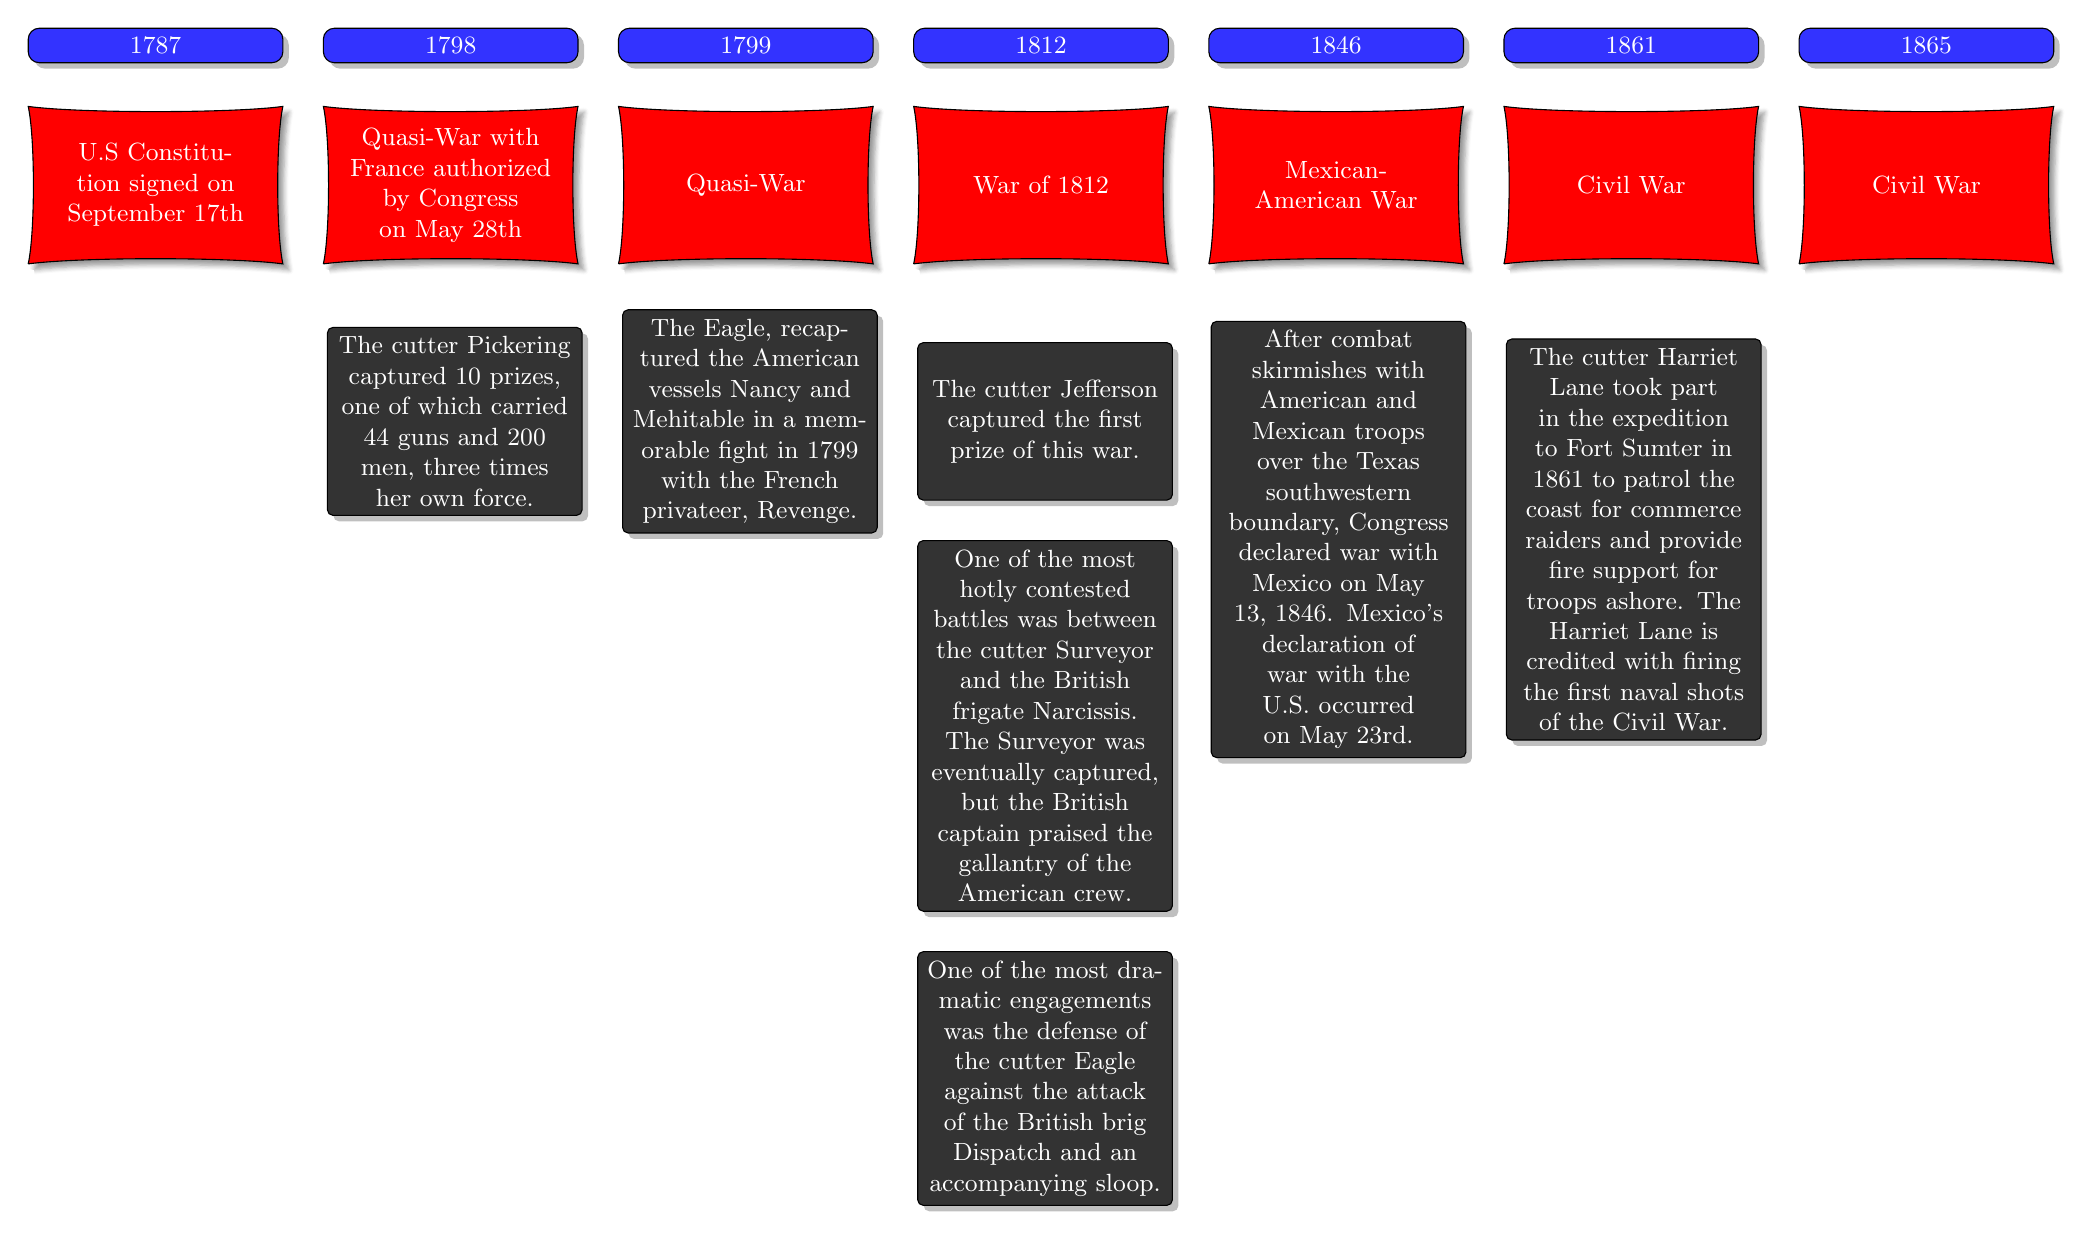
\begin{tikzpicture}[start chain=1 going right, start chain=2 going right,start chain=3 going right,
			node distance=5mm]
\node [box1, on chain=1]{1787};
\node [box1, on chain=1]{1798};
\node [box1, on chain=1]{1799};
\node [box1, on chain=1]{1812};
\node [box1, on chain=1]{1846};
\node [box1, on chain=1]{1861};
\node [box1, on chain=1]{1865};
\node [b1, on chain=2]at (0, -2){U.S Constitution signed on September 17th};
\node [b1, on chain=2] {Quasi-War with France authorized by Congress on May 28th};
\node [b1, on chain=2] {Quasi-War};
\node [b1, on chain=2] {War of 1812};
\node [b1, on chain=2] {Mexican-American War};
\node [b1, on chain=2] {Civil War};
\node [b1, on chain=2] {Civil War};
\node [point, on chain=3]at (3.8,-5) {The cutter Pickering captured 10 prizes, one of which carried 44 guns
and 200 men, three times her own force.};
\node [point, on chain=3]{The Eagle, recaptured the American vessels
Nancy and Mehitable in a memorable fight in 1799 with the French
privateer, Revenge.};
\node [point, on chain=3]{The cutter Jefferson
captured the first prize of this war.};
\node [point, on chain=going below] {One of the most hotly contested battles was between the cutter
Surveyor and the British frigate Narcissis. The Surveyor was
eventually captured, but the British captain praised the gallantry of the
American crew.
};
\node [point, on chain=going below]{One of the most dramatic engagements was the defense of the cutter
Eagle against the attack of the British brig Dispatch and an
accompanying sloop.
};
\node [point, on chain=3]at (12.9, -6.5) {After combat skirmishes with American and Mexican troops over the
Texas southwestern boundary, Congress declared war with Mexico on
May 13, 1846. Mexico’s declaration of war with the U.S. occurred on
May 23rd.
};
\node [point, on chain=3]{The cutter
Harriet Lane took part in the expedition to Fort Sumter in 1861 to patrol
the coast for commerce raiders and provide fire support for troops ashore.
The Harriet Lane is credited with firing the first naval shots of the Civil
War.
};

\end{tikzpicture}
\clearpage
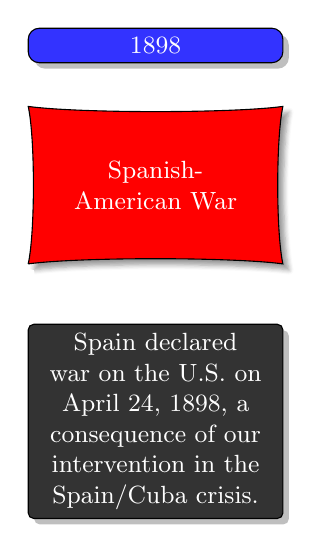
\begin{tikzpicture}[start chain=4 going right, start chain=5 going right, start chain=6 going right, node distance=5mm]
\node [box1, on chain=4]{1898};
\node [b1, on chain=5]at (0,-2) {Spanish-American War};
\node [point, on chain=6] at (0,-5){Spain declared war on the U.S. on April 24, 1898, a consequence of our
intervention in the Spain/Cuba crisis.
};


\end{tikzpicture}

\end{document}
